%%%%%%%%%%%%%%%%%%%%%%%%%%%%% Define Article %%%%%%%%%%%%%%%%%%%%%%%%%%%%%%%%%%
\documentclass{article}
%%%%%%%%%%%%%%%%%%%%%%%%%%%%%%%%%%%%%%%%%%%%%%%%%%%%%%%%%%%%%%%%%%%%%%%%%%%%%%%

%%%%%%%%%%%%%%%%%%%%%%%%%%%%% Using Packages %%%%%%%%%%%%%%%%%%%%%%%%%%%%%%%%%%
\usepackage{geometry}
\usepackage{graphicx}
\usepackage{amssymb}
\usepackage{amsmath}
\usepackage{amsthm}
\usepackage{empheq}
\usepackage{mdframed}
\usepackage{booktabs}
\usepackage{lipsum}
\usepackage{graphicx}
\usepackage{color}
\usepackage{psfrag}
\usepackage{pgfplots}
\usepackage{bm}
%%%%%%%%%%%%%%%%%%%%%%%%%%%%%%%%%%%%%%%%%%%%%%%%%%%%%%%%%%%%%%%%%%%%%%%%%%%%%%%

% Other Settings

%%%%%%%%%%%%%%%%%%%%%%%%%% Page Setting %%%%%%%%%%%%%%%%%%%%%%%%%%%%%%%%%%%%%%%
\geometry{a4paper}

%%%%%%%%%%%%%%%%%%%%%%%%%% Define some useful colors %%%%%%%%%%%%%%%%%%%%%%%%%%
\definecolor{ocre}{RGB}{243,102,25}
\definecolor{mygray}{RGB}{243,243,244}
\definecolor{deepGreen}{RGB}{26,111,0}
\definecolor{shallowGreen}{RGB}{235,255,255}
\definecolor{deepBlue}{RGB}{61,124,222}
\definecolor{shallowBlue}{RGB}{235,249,255}
%%%%%%%%%%%%%%%%%%%%%%%%%%%%%%%%%%%%%%%%%%%%%%%%%%%%%%%%%%%%%%%%%%%%%%%%%%%%%%%

%%%%%%%%%%%%%%%%%%%%%%%%%% Define an orangebox command %%%%%%%%%%%%%%%%%%%%%%%%
\newcommand\orangebox[1]{\fcolorbox{ocre}{mygray}{\hspace{1em}#1\hspace{1em}}}
%%%%%%%%%%%%%%%%%%%%%%%%%%%%%%%%%%%%%%%%%%%%%%%%%%%%%%%%%%%%%%%%%%%%%%%%%%%%%%%

%%%%%%%%%%%%%%%%%%%%%%%%%%%% English Environments %%%%%%%%%%%%%%%%%%%%%%%%%%%%%
\newtheoremstyle{mytheoremstyle}{3pt}{3pt}{\normalfont}{0cm}{\rmfamily\bfseries}{}{1em}{{\color{black}\thmname{#1}~\thmnumber{#2}}\thmnote{\,--\,#3}}
\newtheoremstyle{myproblemstyle}{3pt}{3pt}{\normalfont}{0cm}{\rmfamily\bfseries}{}{1em}{{\color{black}\thmname{#1}~\thmnumber{#2}}\thmnote{\,--\,#3}}
\theoremstyle{mytheoremstyle}
\newmdtheoremenv[linewidth=1pt,backgroundcolor=shallowGreen,linecolor=deepGreen,leftmargin=0pt,innerleftmargin=20pt,innerrightmargin=20pt,]{theorem}{Theorem}[section]
\theoremstyle{mytheoremstyle}
\newmdtheoremenv[linewidth=1pt,backgroundcolor=shallowBlue,linecolor=deepBlue,leftmargin=0pt,innerleftmargin=20pt,innerrightmargin=20pt,]{definition}{Definition}[section]
\theoremstyle{myproblemstyle}
\newmdtheoremenv[linecolor=black,leftmargin=0pt,innerleftmargin=10pt,innerrightmargin=10pt,]{problem}{Problem}[section]
%%%%%%%%%%%%%%%%%%%%%%%%%%%%%%%%%%%%%%%%%%%%%%%%%%%%%%%%%%%%%%%%%%%%%%%%%%%%%%%

%%%%%%%%%%%%%%%%%%%%%%%%%%%%%%% Plotting Settings %%%%%%%%%%%%%%%%%%%%%%%%%%%%%
\usepgfplotslibrary{colorbrewer}
\pgfplotsset{width=8cm,compat=1.9}
%%%%%%%%%%%%%%%%%%%%%%%%%%%%%%%%%%%%%%%%%%%%%%%%%%%%%%%%%%%%%%%%%%%%%%%%%%%%%%%

%%%%%%%%%%%%%%%%%%%%%%%%%%%%%%% Title & Author %%%%%%%%%%%%%%%%%%%%%%%%%%%%%%%%
\title{Hyperbolic Trigonometric Functions}
\author{Patrick Chen}
\date{Oct 2, 2024}
%%%%%%%%%%%%%%%%%%%%%%%%%%%%%%%%%%%%%%%%%%%%%%%%%%%%%%%%%%%%%%%%%%%%%%%%%%%%%%%

\newcommand{\sech}{\text{sech}}
\newcommand{\csch}{\text{csch}}

\begin{document}
    \maketitle
    Hyperbolic trigonometric functions describe points on a hyperbola. The graph
    of a hyperbola satisfies $x^2-y^2=1$ and points on the hyperbola can be
    described as $(\cosh x, \sinh x)$ in the same way points on a circle can be
    described as $(\cos t, \sin t)$

    \begin{align*}
        \sinh x = \frac{e^x-e^{-x}}{2} \\
        \cosh x = \frac{e^x+e^{-x}}{2} \\
        \tanh x = \frac{\sinh x}{\cosh x}
    \end{align*}
    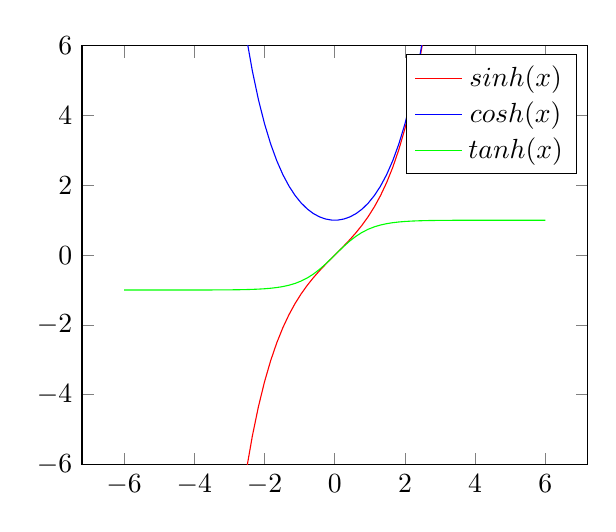
\begin{tikzpicture}
        \begin{axis} [ymin=-6, ymax=6]
             \addplot [
                domain=-6:6,
                samples=70,
                color=red,
                ]
                {sinh(x)};
            \addlegendentry{$sinh(x)$}
            \addplot [
                domain=-6:6,
                samples=70,
                color=blue,
                ]
                {cosh(x)};
            \addlegendentry{$cosh(x)$}
            \addplot [
                domain=-6:6,
                samples=70,
                color=green,
                ]
                {tanh(x)};
            \addlegendentry{$tanh(x)$}
         \end{axis}
    \end{tikzpicture}

    \begin{align*}
        \cosh^2x - \sinh^2x = 1 \\
        (\frac{e^x+e^{-x}}{2})^2 - (\frac{e^x-e^{-x}}{2})^2 \\
        \frac{(e^x+e^{-x})^2 - (e^x-e^{-x})^2}{4} \\
        \frac{(e^{2x} + 2e^xe^{-x} +e^{-2x}) - (e^{2x} - 2e^xe^{-x} +e^{-2x})}{4} \\
        \frac{2-(-2)}{4} \\
        1
    \end{align*}

    \subsection*{Identities}
    \begin{align*}
        \sinh(-x)               &= -\sinh x \\
        \cosh(-x)               &= \cosh x \\
        \cosh^2 x - \sinh^2 x   &= 1 \\
        1-\tanh^2 x             &= \sech^2 x \\
        \sinh(x+y)              &= \sinh x \cosh y + \cosh x \sinh y \\
        \cosh(x+y)              &= \cosh x \cosh y + \sinh x \sinh y
    \end{align*}

    \begin{align*}
        1 - \tanh^2 x = \sech^2x \\
        \frac{\cosh^2 x}{\cosh^2 x} - \frac{\sinh^2 x}{\cosh^2 x} = \sech^2x \\
        \frac{\cosh^2 x - \sinh^2 x}{\cosh^2 x} = \sech^2x \\
        \frac{1}{\cosh^2 x} = \sech^2x \\
        \sech^2 x = \sech^2 x
    \end{align*}

    \section*{Derivatives of Hyperbolic Trigonometric Functions}
    \begin{align*}
        \frac{d}{dx} (\sinh x) &= \cosh x \\
        \frac{d}{dx} (\cosh x) &= \sinh x \\
        \frac{d}{dx} (\tanh x) &= \sech^2 x \\
        \frac{d}{dx} (\csch x) &= -\csch x \coth x \\
        \frac{d}{dx} (\sech x) &= -\sech x \tanh x \\
        \frac{d}{dx} (\coth x) &= -\csch^2 x
    \end{align*}
    \begin{align*}
        y &= \sinh x \\
        \frac{dy}{dx} &= \frac{d}{dx} (\frac{1}{2})(e^x-e^{-x}) \\
             &=  (\frac{1}{2})(\frac{d}{dx} e^x - \frac{d}{dx} e^{-x}) \\
             &=  (\frac{1}{2})(e^x - (- e^{-x})) \\
             &=  (\frac{1}{2})(e^x + e^{-x}) \\
             &= \cosh x
    \end{align*}

    \subsection*{One to one and derivatives}
    If a function's derivative is always positive or always negative for all
    points, then it is one-to-one. Since $\frac{d}{dx} \sinh  x = \cosh x$, and
    $\cosh x$ is always positive, $\sinh$ is always positive and one-to-one.

    \section*{Inverse}
    Inverse of $\sinh x$
    \begin{align*}
        \sinh x = \frac{e^x-e^{-x}}{2} \\
        y = \frac{e^x-e^{-x}}{2} \\
        2y = e^x-e^{-x} \\
        2y = e^x(1 - e^{-2x}) \\
        2ye^{-x} = 1 - e^{-2x} \\
        2ye^{-x} + e^{-2x} = 1 \\
        (e^{-x})^2 + 2y(e^{-x}) - 1 = 0 \\
        e^{-x} = -y \pm \sqrt{y^2+1} \\
        x = -\ln\big(-y \pm \sqrt{y^2+1}\big) \\
        x = -\ln\big(-y - \sqrt{y^2+1}\big) \\
    \end{align*}

\end{document}
